% questions.tex —— 2010 年·普通高等学校招生考试·湖南卷·理科 · 题目内容片段（无答案）
% 由 tools/generate_projects.py 依来源总账自 2010/2010_数学真题_湖南理_试题.md 生成，勿手改（改源 MD 后重跑）
状态：needs-review；依固定候选 PDF 两页（印刷页 601–602）逐题核验，六幅图已矢量重绘。原页未印分值，不补。
\gkpart{一、选择题}
\begin{question}
\gkti{1}已知集合 $M=\{1,2,3\}$，$N=\{2,3,4\}$，则（　）

（A）$M\subseteq N$

（B）$N\subseteq M$

（C）$M\cap N=\{2,3\}$

（D）$M\cup N=\{1,4\}$

\end{question}
\begin{question}
\gkti{2}下列命题中是假命题的是（　）

（A）$\forall x\in\mathbf R$，$2^{x-1}>0$

（B）$\forall x\in\mathbf N^*$，$(x-1)^2>0$

（C）$\exists x\in\mathbf R$，$\lg x<1$

（D）$\exists x\in\mathbf R$，$\tan x=2$

\end{question}
\begin{question}
\gkti{3}极坐标方程 $\rho=\cos\theta$ 和参数方程 $\begin{cases}x=-1-t,\\ y=2+3t\end{cases}$（$t$ 为参数）所表示的图形分别是（　）

（A）圆、直线

（B）直线、圆

（C）圆、圆

（D）直线、直线

\end{question}
\begin{question}
\gkti{4}在 $\mathrm{Rt}\triangle ABC$ 中，$\angle C=90^\circ$，$AC=4$，则 $\overrightarrow{AB}\cdot\overrightarrow{AC}$ 等于（　）

（A）$-16$

（B）$-8$

（C）$8$

（D）$16$

\end{question}
\begin{question}
\gkti{5}$\displaystyle\int_2^4\frac1x\,\mathrm dx$ 等于（　）

（A）$-2\ln2$

（B）$2\ln2$

（C）$-\ln2$

（D）$\ln2$

\end{question}
\begin{question}
\gkti{6}在 $\triangle ABC$ 中，角 $A$，$B$，$C$ 所对的边长分别为 $a$，$b$，$c$，若 $\angle C=120^\circ$，$c=\sqrt2a$，则（　）

（A）$a>b$

（B）$a<b$

（C）$a=b$

（D）$a$ 与 $b$ 的大小关系不能确定

\end{question}
\begin{question}
\gkti{7}在某种信息传输过程中，用 $4$ 个数字的一个排列（数字允许重复）表示一个信息，不同排列表示不同信息，若所用数字只有 $0$ 和 $1$，则与信息 $0110$ 至多有两个对应位置上的数字相同的信息个数为（　）

（A）$10$

（B）$11$

（C）$12$

（D）$15$

\end{question}
\begin{question}
\gkti{8}用 $\min\{a,b\}$ 表示 $a$，$b$ 两数中的最小值。若函数 $f(x)=\min\{|x|,|x+t|\}$ 的图象关于直线 $x=-\dfrac12$ 对称，则 $t$ 的值为（　）

（A）$-2$

（B）$2$

（C）$-1$

（D）$1$

\end{question}
\gkpart{二、填空题}
\begin{question}
\gkti{9}已知一种材料的最佳加入量在 $110$ g 到 $210$ g 之间。若用 $0.618$ 法安排实验，则第一次试点的加入量可以是 $\underline{\qquad}$ g。

\Needspace{0.4\textheight}
\end{question}
\begingroup
\renewenvironment{question}{\Needspace{0.5\textheight}}{}
\begin{question}
\gkti{10}如图所示，过 $\odot O$ 外一点 $P$ 作一条直线与 $\odot O$ 交于 $A$，$B$ 两点。已知 $PA=2$，点 $P$ 到 $\odot O$ 的切线长 $PT=4$，则弦 $AB$ 的长为 $\underline{\qquad}$。
\nopagebreak[4]
\begin{center}% 2010 年湖南卷理科第 10 题：⊙O 外一点 P 的切线与割线。
% 来源 PDF：普通高考/2010/2010湖南理.pdf，SHA-256 db6274a80ebb0022ff1b91b2cd3714fe8cca335e48be69805dcd87cdefd8c8d1。
% 原页：第 1 页（A3 三栏）第 2 栏上部，书页码 601。
% 重绘依据：照原页，圆心 O 在圆内偏右上；P 在圆外左下，PT 为切线（T 在圆左上），
%   割线自 P 向右穿过圆于 A（近 P）与 B（远 P），A、B 在圆上，弦 AB 近似水平。
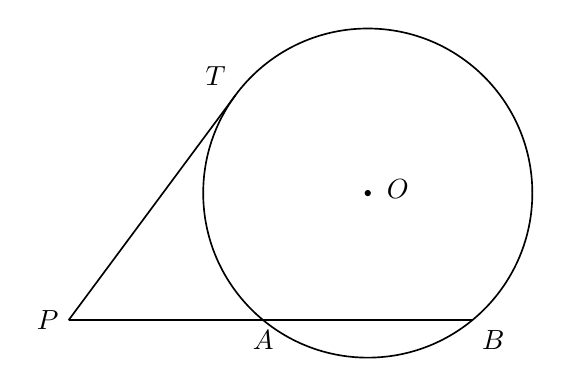
\begin{tikzpicture}[scale=0.95, semithick]
  \coordinate (O) at (0,0);
  \coordinate (P) at (-4,-1.7);
  \coordinate (T) at (-1.767,1.31);
  \coordinate (A) at (-1.396,-1.7);
  \coordinate (B) at (1.396,-1.7);

  \draw (O) circle (2.2);
  \fill (O) circle (1.2pt);
  \node[right] at (0.12,0.06) {$O$};

  \draw (P) -- (T);
  \draw (P) -- (B);

  \node[above left] at (T) {$T$};
  \node[left] at (P) {$P$};
  \node[below] at (A) {$A$};
  \node[below right] at (B) {$B$};
\end{tikzpicture}
\end{center}
\nopagebreak[4]
\end{question}
\endgroup
\begin{question}
\gkti{11}在区间 $[-1,2]$ 上随机取一个数 $x$，则 $|x|\leqslant1$ 的概率为 $\underline{\qquad}$。

\Needspace{0.4\textheight}
\end{question}
\begingroup
\renewenvironment{question}{\Needspace{0.5\textheight}}{}
\begin{question}
\gkti{12}如图是求 $1^2+2^2+3^2+\cdots+100^2$ 的值的程序框图，则正整数 $n=$ $\underline{\qquad}$。
\nopagebreak[4]
\begin{center}% 2010 年湖南卷理科第 12 题：求 1^2+2^2+...+100^2 的程序框图。
% 来源 PDF：普通高考/2010/2010湖南理.pdf，SHA-256 db6274a80ebb0022ff1b91b2cd3714fe8cca335e48be69805dcd87cdefd8c8d1。
% 原页：第 1 页（A3 三栏）第 2 栏中部，书页码 601。
% 重绘依据：照原页，开始→i=1,s=0→判断 i<=n?；判断框「是」向右、向上依次经
%   s=s+i^2、i=i+1 后向左汇入主干（即在判断前先累加再自增）；「否」向下经输出 s 到结束。
\begin{tikzpicture}[scale=1.0, semithick,
  every node/.style={inner sep=2pt},
  box/.style={draw, minimum width=2.6cm, minimum height=0.6cm, align=center},
  round/.style={draw, rounded corners=6pt, minimum width=1.5cm,
    minimum height=0.6cm, align=center},
  para/.style={draw, trapezium, trapezium left angle=70, trapezium right angle=110,
    minimum width=2.2cm, minimum height=0.65cm, align=center},
  dec/.style={draw, diamond, aspect=2.4, minimum width=2.8cm,
    minimum height=1.1cm, align=center},
  arr/.style={->, >=stealth}]

  \node[round] (start) at (0,9.1) {开始};
  \node[box]   (init)  at (0,8.1) {$i=1,\ s=0$};
  \node[dec]   (test)  at (0,4.9) {$i\leqslant n$?};
  \node[para]  (out)   at (0,3.0) {输出 $s$};
  \node[round] (end)   at (0,1.9) {结束};

  \node[box] (sum) at (3.5,5.9) {$s=s+i^2$};
  \node[box] (inc) at (3.5,7.2) {$i=i+1$};

  \draw[arr] (start) -- (init);
  \draw[arr] (init) -- (test);
  \draw[arr] (test.south) -- (out.north);
  \node[right] at (0.14,3.85) {否};
  \draw[arr] (out) -- (end);

  \draw[arr] (test.east) -| (sum.south);
  \node[right] at (1.75,5.08) {是};
  \draw[arr] (sum.north) -- (inc.south);
  \draw[arr] (inc.west) -- (0,7.2);
\end{tikzpicture}
\end{center}
\nopagebreak[4]
\Needspace{0.4\textheight}
\end{question}
\endgroup
\begingroup
\renewenvironment{question}{\Needspace{0.5\textheight}}{}
\begin{question}
\gkti{13}图中的三个直角三角形是一个体积为 $20$ cm$^3$ 的几何体的三视图，则 $h=$ $\underline{\qquad}$ cm。
\nopagebreak[4]
\begin{center}% 2010 年湖南卷理科第 13 题：体积 20 cm^3 的几何体的三视图。
% 来源 PDF：普通高考/2010/2010湖南理.pdf，SHA-256 db6274a80ebb0022ff1b91b2cd3714fe8cca335e48be69805dcd87cdefd8c8d1。
% 原页：第 1 页（A3 三栏）第 2 栏下部，书页码 601。
% 重绘依据：三个直角三角形——正视图直角边 5 与 h（直角在左下），
%   侧视图直角边 6 与 h（直角在左下），俯视图直角边 5、6（直角在左上）；
%   俯视图在原页未标数字，此处亦不标。图中 h 按原页比例虚设，不代表答案。
\begin{tikzpicture}[scale=0.62, semithick]
  % 正视图：宽 5，高 h
  \draw (0,0) -- (5,0) -- (0,3.2) -- cycle;
  \draw[<->] (-0.6,0) -- (-0.6,3.2);
  \draw (-0.75,0) -- (-0.35,0);
  \draw (-0.75,3.2) -- (-0.35,3.2);
  \node[left] at (-0.85,1.6) {$h$};
  \draw[<->] (0,-0.6) -- (5,-0.6);
  \draw (0,-0.75) -- (0,-0.35);
  \draw (5,-0.75) -- (5,-0.35);
  \node[below] at (2.5,-0.55) {$5$};
  \node[below] at (2.5,-1.45) {正视图};

  % 侧视图：宽 6，高 h
  \draw (7.6,0) -- (13.6,0) -- (7.6,3.2) -- cycle;
  \draw[<->] (7.6,-0.6) -- (13.6,-0.6);
  \draw (7.6,-0.75) -- (7.6,-0.35);
  \draw (13.6,-0.75) -- (13.6,-0.35);
  \node[below] at (10.6,-0.55) {$6$};
  \node[below] at (10.6,-1.45) {侧视图};

  % 俯视图：宽 5，高 6，直角在左上
  \draw (0,-4.6) -- (5,-4.6) -- (0,-10.6) -- cycle;
  \node[below] at (2.5,-10.9) {俯视图};
\end{tikzpicture}
\end{center}
\nopagebreak[4]
\end{question}
\endgroup
\begin{question}
\gkti{14}过抛物线 $x^2=2py$（$p>0$）的焦点作斜率为 $1$ 的直线与该抛物线交于 $A$，$B$ 两点，$A$，$B$ 在 $x$ 轴上的正射影分别为 $D$，$C$。若梯形 $ABCD$ 的面积为 $12\sqrt2$，则 $p=$ $\underline{\qquad}$。

\end{question}
\begin{question}
\gkti{15}若数列 $\{a_n\}$ 满足：对任意的 $n\in\mathbf N^*$，只有有限个正整数 $m$ 使得 $a_m<n$ 成立，记这样的 $m$ 的个数为 $(a_n)^*$，则得到一个新数列 $\{(a_n)^*\}$。例如，若数列 $\{a_n\}$ 是 $1,2,3,\cdots,n,\cdots$，则数列 $\{(a_n)^*\}$ 是 $0,1,2,\cdots,n-1,\cdots$。已知对任意的 $n\in\mathbf N^*$，$a_n=n^2$，则 $(a_5)^*=$ $\underline{\qquad}$，$((a_n)^*)^*=$ $\underline{\qquad}$。

\end{question}
\gkpart{三、解答题}
\begin{question}
\gkti{16}已知函数 $f(x)=\sqrt3\sin2x-2\sin^2x$。

（1）求函数 $f(x)$ 的最大值；

（2）求函数 $f(x)$ 的零点的集合。

\Needspace{0.4\textheight}
\end{question}
\begingroup
\renewenvironment{question}{\Needspace{0.5\textheight}}{}
\begin{question}
\gkti{17}如图，是某城市通过抽样得到的居民某年的月均用水量（单位：吨）的频率分布直方图。

（1）求直方图中 $x$ 的值；

（2）若将频率视为概率，从这个城市随机抽取 $3$ 位居民（看作有放回的抽样），求月均用水量在 $3$ 至 $4$ 吨的居民数 $X$ 的分布列和数学期望。
\nopagebreak[4]
\begin{center}% 2010 年湖南卷理科第 17 题：月均用水量的频率分布直方图。
% 来源 PDF：普通高考/2010/2010湖南理.pdf，SHA-256 db6274a80ebb0022ff1b91b2cd3714fe8cca335e48be69805dcd87cdefd8c8d1。
% 原页：第 1 页（A3 三栏）第 3 栏中部，书页码 601。
% 重绘依据：组距 1，五组 [0,1]、[1,2]、[2,3]、[3,4]、[4,5] 的高度依次为
%   x、0.37、0.39、0.1、0.02；纵轴标「频率/组距」，横轴标「月均用水量/吨」；
%   0.39、0.37、0.1、0.02 以虚线引到对应矩形条顶部。
\begin{tikzpicture}[x=1.2cm, y=10cm, semithick, font=\scriptsize]
  \draw[->] (0,0) -- (8.4,0);
  \draw[->] (0,0) -- (0,0.55);
  \node[anchor=west, font=\small] at (0.04,0.535) {频率};
  \node[anchor=west, font=\small] at (0.04,0.492) {组距};

  % 五个矩形条（组距 1）
  \draw (0,0) rectangle (1,0.12);
  \draw (1,0) rectangle (2,0.37);
  \draw (2,0) rectangle (3,0.39);
  \draw (3,0) rectangle (4,0.10);
  \draw (4,0) rectangle (5,0.02);

  % 横轴刻度
  \foreach \k in {0,1,2,3,4,5} {
    \draw (\k,0) -- ++(0,-0.008);
    \node[below] at (\k,-0.010) {\k};
  }
  \node[anchor=west, font=\small] at (5.35,-0.012) {月均用水量/吨};

  % 纵轴读数与虚线
  \draw[dashed] (0,0.39) -- (2,0.39);
  \draw[dashed] (0,0.37) -- (1,0.37);
  \draw[dashed] (0,0.10) -- (3,0.10);
  \draw[dashed] (0,0.02) -- (4,0.02);
  \node[left] at (0,0.405) {0.39};
  \node[left] at (0,0.37) {0.37};
  \node[left] at (0,0.12) {$x$};
  \node[left] at (0,0.10) {0.1};
  \node[left] at (0,0.02) {0.02};
\end{tikzpicture}
\end{center}
\nopagebreak[4]
\Needspace{0.4\textheight}
\end{question}
\endgroup
\begingroup
\renewenvironment{question}{\Needspace{0.5\textheight}}{}
\begin{question}
\gkti{18}如图所示，在正方体 $ABCD-A_1B_1C_1D_1$ 中，$E$ 是棱 $DD_1$ 的中点。

（1）求直线 $BE$ 和平面 $ABB_1A_1$ 所成的角的正弦值；

（2）在棱 $C_1D_1$ 上是否存在一点 $F$，使 $B_1F\parallel$ 平面 $A_1BE$？证明你的结论。
\nopagebreak[4]
\begin{center}% 2010 年湖南卷理科第 18 题：正方体 ABCD-A1B1C1D1，E 为棱 DD1 的中点。
% 来源 PDF：普通高考/2010/2010湖南理.pdf，SHA-256 db6274a80ebb0022ff1b91b2cd3714fe8cca335e48be69805dcd87cdefd8c8d1。
% 原页：第 2 页（A3 三栏）第 1 栏上部，书页码 602。
% 重绘依据：照原页斜二测画法，前面 BB1C1C，后面 AA1D1D 向右上平移；
%   实线为可见棱，虚线为被遮挡的三条棱 AA1、AB、AD；
%   另以虚线画出辅助三角形 A1BE（A1B、BE、A1E），E 在 D1D 上且为其中点。
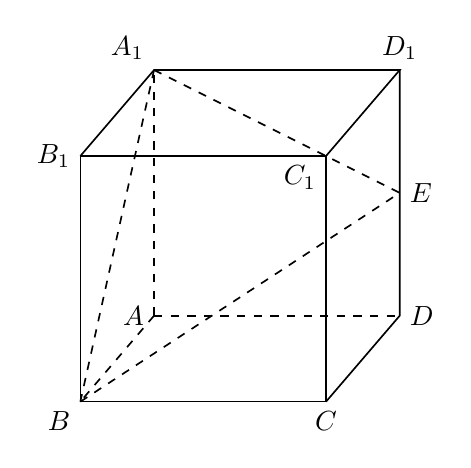
\begin{tikzpicture}[scale=0.78, semithick]
  \coordinate (B)  at (0,0);
  \coordinate (C)  at (4,0);
  \coordinate (C1) at (4,4);
  \coordinate (B1) at (0,4);
  \coordinate (A)  at (1.2,1.4);
  \coordinate (D)  at (5.2,1.4);
  \coordinate (A1) at (1.2,5.4);
  \coordinate (D1) at (5.2,5.4);
  \coordinate (E)  at (5.2,3.4);

  % 可见棱
  \draw (B) -- (C) -- (C1) -- (B1) -- cycle;
  \draw (B1) -- (A1) -- (D1) -- (C1);
  \draw (D1) -- (D) -- (C);

  % 被遮挡的棱
  \draw[dashed] (A) -- (B);
  \draw[dashed] (A) -- (D);
  \draw[dashed] (A) -- (A1);

  % 辅助线：三角形 A1BE
  \draw[dashed] (A1) -- (B);
  \draw[dashed] (B) -- (E);
  \draw[dashed] (A1) -- (E);

  \node[below left]  at (B)  {$B$};
  \node[below]       at (C)  {$C$};
  \node[left]        at (B1) {$B_1$};
  \node[below left]  at (C1) {$C_1$};
  \node[above left]  at (A1) {$A_1$};
  \node[above]       at (D1) {$D_1$};
  \node[left]        at (A)  {$A$};
  \node[right]       at (D)  {$D$};
  \node[right]       at (E)  {$E$};
\end{tikzpicture}
\end{center}
\nopagebreak[4]
\Needspace{0.4\textheight}
\end{question}
\endgroup
\begingroup
\renewenvironment{question}{\Needspace{0.5\textheight}}{}
\begin{question}
\gkti{19}为了考察冰川的融化状况，一支科考队在某冰川上相距 $8$ km 的 $A$，$B$ 两点各建一个考察基地。视冰川面为平面形，以过 $A$，$B$ 两点的直线为 $x$ 轴，线段 $AB$ 的垂直平分线为 $y$ 轴建立平面直角坐标系（如图）。在直线 $x=2$ 的右侧，考察范围为到点 $B$ 的距离不超过 $\dfrac{6\sqrt5}{5}$ km 的区域；在直线 $x=2$ 的左侧，考察范围为到 $A$，$B$ 两点的距离之和不超过 $4\sqrt5$ km 的区域。

（1）求考察区域边界曲线的方程；

（2）如图所示，设线段 $P_1P_2$，$P_2P_3$ 是冰川的部分边界线（不考虑其他边界），当冰川融化时，边界线沿与其垂直的方向朝考察区域平行移动，第一年移动 $0.2$ km，以后每年移动的距离为前一年的 $2$ 倍。求冰川边界线移动到考察区域所需的最短时间。
\nopagebreak[4]
\begin{center}% 2010 年湖南卷理科第 19 题：冰川边界与考察区域的平面示意图。
% 来源 PDF：普通高考/2010/2010湖南理.pdf，SHA-256 db6274a80ebb0022ff1b91b2cd3714fe8cca335e48be69805dcd87cdefd8c8d1。
% 原页：第 2 页（A3 三栏）第 1 栏下部，书页码 602。
% 重绘依据：照原页坐标系，A(-4,0)、B(4,0)，冰界线 P1P2（斜线）与 P2P3（水平线），
%   P1(-5√3,-1)、P2(-8√3/3,6)、P3(8,6)；虚线 x=2 为左右两种考察范围的分界；
%   「已融化」「冰川」分列斜界线两侧，「区域」标于 x=2 右侧。
\begin{tikzpicture}[scale=0.62, semithick]
  \draw[->] (-9.8,0) -- (9.8,0) node[right] {$x$};
  \draw[->] (0,-2.6) -- (0,7.7) node[above] {$y$};

  \coordinate (A)  at (-4,0);
  \coordinate (B)  at (4,0);
  \coordinate (P1) at (-8.660,-1);
  \coordinate (P2) at (-4.619,6);
  \coordinate (P3) at (8,6);

  \draw (P1) -- (P2) -- (P3);
  \draw[dashed] (2,-2.4) -- (2,7.5);

  \fill (A) circle (1.2pt);
  \fill (B) circle (1.2pt);
  \fill (P1) circle (1.2pt);
  \fill (P2) circle (1.2pt);
  \fill (P3) circle (1.2pt);

  \node[below left]  at (A)  {$A(-4,0)$};
  \node[below right] at (B)  {$B(4,0)$};
  \node[below left]  at (P1) {$P_1(-5\sqrt3,-1)$};
  \node[left]        at (P2) {$P_2\left(-\dfrac{8\sqrt3}{3},6\right)$};
  \node[right]       at (P3) {$P_3(8,6)$};
  \node[below left]  at (0,0) {$O$};

  \node[below] at (2,-2.45) {$x=2$};

  % 冰川、已融化（沿界线两侧，照原页字位）
  \node at (-7.3,1.9) {已};
  \node at (-6.9,3.1) {融};
  \node at (-6.5,4.3) {化};
  \node at (-1.2,2.2) {冰};
  \node at (6.6,1.4) {川};

  \node at (3.3,6.55) {区域};
\end{tikzpicture}
\end{center}
\nopagebreak[4]
\end{question}
\endgroup
\begin{question}
\gkti{20}已知函数 $f(x)=x^2+bx+c$（$b$，$c\in\mathbf R$），对任意的 $x\in\mathbf R$，恒有 $f'(x)\leqslant f(x)$。

（1）证明：当 $x\geqslant0$ 时，$f(x)\leqslant(x+c)^2$；

（2）若对满足题设条件的任意 $b$，$c$，不等式 $f(c)-f(b)\leqslant M(c^2-b^2)$ 恒成立，求 $M$ 的最小值。

\end{question}
\begin{question}
\gkti{21}数列 $\{a_n\}$（$n\in\mathbf N^*$）中，$a_1=a$，$a_{n+1}$ 是函数 $f_n(x)=\dfrac13x^3-\dfrac12(3a_n+n^2)x^2+3n^2a_nx$ 的极小值点。

（1）当 $a=0$ 时，求通项 $a_n$；

（2）是否存在 $a$，使数列 $\{a_n\}$ 是等比数列？若存在，求 $a$ 的取值范围；若不存在，请说明理由。

\end{question}